\documentclass[10pt,a4paper]{article}
\usepackage[utf8]{inputenc}
\usepackage[finnish]{babel}
\usepackage[T1]{fontenc}
\usepackage{graphicx}

\usepackage{hyperref}

\usepackage{algpseudocode}

\begin{document}

\title{A* ja Dikstra vertailussa}
\author{Matti Nelimarkka}

\setlength{\parindent}{0pt}
\setlength{\parskip}{10pt}

\maketitle

\newpage

\section*{Tehtävänanto}

Toteuta yleinen ohjelma verkon käsittelyä varten, siten että siinä on mahdollisuus säilöä solmuja ja solmujen välisiä kaaria. Verkko tulee voida määritellä ulkoisessa tiedostossa muodossa \texttt{<solmu 1>:<solmu 2>:<etäisyys solmusta 1 solmuun 2>}, esimerkiksi:

\begin{verbatim}
a:b:5
a:c:10
a:d:1
c:b:4
d:c:10
\end{verbatim}

Lisäksi toteuta lyhyimmän polun etsintä sekä Dikstran algoritmilla \cite{dikstra} että A*-algoritmilla \cite{astar}. Vertaa näitä kahta toteutustapaa toisiinsa empiirisesti.

\section{Toteutus}

Ohjelma on toteutettu oliomallinnusta hyödyntäen: paketteja, rajapintoja ja perintäsuhteita on käytetty selkeyttämään ohjelman rakennetta. Ohjelma koostuu neljästä paketista

\begin{description}
\item[datastructures] sisältää ohjelman toiminnan kannalta välttämättömät itse toteutetut tietorakenteet kekoa, hajautustaulua ja listaa varten. Tarkemmin tätä pakettia käsitellään kappaleessa \ref{datastructures}.
\item[model] sisältää ohjelman tarvitsemat itsenäiset toteutustietorakenteet, yleisen muodon verkon sekä erityiset versiot verkosta, jotka toteuttavat tutkittava olevat Dikstran sekä A*-algoritmit. Yleistä verkkoa on esitelty tarkemmin kappaleessa \ref{model.graph} ja lyhyimmän polun etsintää kappaleessa \ref{path}.
\item[io] tarjoaa palveluja tiedoston lukemiseen tekstiformaatista ohjelman ymmärtämäksi verkoksi. Tätä käsitellään kappaleessa \ref{io}.
\item[test] sisältää ohjelman muiden luokkien testaamiseen tarvittavat luokat. Ohjelman jokaiselle luokalle on kirjoitettu yksikkötestit. Testausprosessia on käsitelty tarkemmin kappaleessa \ref{test}.
\end{description}


\subsection{Omat tietorakenteet}
\label{datastructures}

Tietorakenteiden harjoitustyön luonteen vuoksi toteutukseen on kuulunut omien tietorakenteiden kehittäminen ja testaaminen. Käytännöllisistä syistä johtuen tietorakenteeni vastaavat \texttt{java.util}-paketin tietorakenteita, koska tämä mahdollisti ketterämmän kehityksen\footnote{Muuttujat on määritelty yleisten rajapintojen kautta, jolloin niiden implementaatioluokat pystyi helposti vaihtamaan Javan rajapintaa toteuttavasta luokasta omaan toteutukseeni.} ja Javan valmiiden toiminnallisuuksien käytön osana ohjelmaa. Täsmällisesti toteutussuhteet on esitetty taulukossa \ref{omat_tietorakenteet}.

\begin{table}

\begin{tabular}{l|l}
Toteuttava luokka & Rajapinta \\ 
\hline 
\texttt{MyMap} &  \href{http://docs.oracle.com/javase/6/docs/api/java/util/Map.html}{\texttt{java.util.Map}} \\
\texttt{MyHeap} & \href{http://docs.oracle.com/javase/6/docs/api/java/util/Queue.html}{\texttt{java.util.Queue}} \\ 
\texttt{MyList} & \href{http://docs.oracle.com/javase/6/docs/api/java/util/List.html}{\texttt{java.util.List}} \\ 
\texttt{MySet} & \href{http://docs.oracle.com/javase/6/docs/api/java/util/Set.html}{\texttt{java.util.Set}} \\ 
\texttt{MyIterator} & \href{http://docs.oracle.com/javase/6/docs/api/java/util/ListIterator.html}{\texttt{java.util.ListIterator}} \\ 
\end{tabular}
\caption{Omien tietorakenteiden vastaavuus Javan tietorakenteiden kanssa}
\label{omat_tietorakenteet}
\end{table}

Hajautustaulun toteuttaa luokka \texttt{MyMap}, sen sisäinen toteutus on käyttää ylivuotolistoja törmäysten hallintaan. Täyttöasteeksi sallitaan 90 \%, minkä jälkeen taulun kokoa kasvatetaan ja alkiot uudelleenhajautetaan. Tällä asetuksella suurta määrää törmäyksiä ei pitäisi tapahtua, olettaen, että hajautusfunktio jakaa arvoja tasaisesti koko alueelle. Tällöin saavutetaan\footnote{Laskennallisesti usein myös huomioidaan mahdolliset ylivuodot, jolloin keskimääräiseksi suoritusajaksi esitetään tarkempi $\mathcal{O}(n) = 1 + \frac{n}{k}$.} $\mathcal{O}(n) = 1$-suoritusaika operaatioille avaimen lisäys, avainta vastaavan arvon hakeminen ja avaimen olemassaolon tarkistaminen. Vastaavasti operaatiot kaikkien arvojen hakemiseen, kaikkien avainten hakemiseen sekä alkioiden lukumäärän laskemiseen ovat lineaarisia. Tilankäyttö on myös lineraarinen.

Minimikeon toteuttaa luokka \texttt{MyHeap}, sen sisäinen toteutus on binäärikeko, mikä mahdollistaa alkion lisäämisen ja poistamisen ajassa $\mathcal{O}(n) = \log n$. Pienimmän arvon noutaminen, alkioiden lukumäärän sekä tyhjyyden tarkistaminen suoritaan vakioajassa. Tilankäyttö on lineaarinen.

Listan toteuttaa luokka \texttt{MyList}. Sisäiseksi toteutukseksi valittiin tunnusalkiollinen yksisuuntainen linkitetty lista. Tunnussolmuksellisuus tekee toteuksesta helpompaa, ja yksisuuntainen linkitys oli luonteva valinta: ainoastaan poisto-operaatiossa olisi hyötyä kaksisuuntaisesta linkityksestä, eikä siinäkään tapauksessa saavutettaisi lineaarisuutta parempaa suoritusaikaa. Olen lisännyt toteutukseen myös tunnusalkion loppuun, mikä mahdollistaa uuden alkion lisäämisen vakioajassa. Alkion hakeminen tietystä indeksistä, alkion olemassa olon tarkastelu sekä poistaminen suoriutuvat lineaarisessa ajassa, koska yksittäisen alkion hakeminen \texttt{getElement(int arg0)}-metodilla on lineaarinen. Tilankäyttö on lineraarinen.

Sekä \texttt{MySet} että \texttt{MyIterator} on toteutettu Javan rajapintavaatimusten johdosta. Molemmat käyttävät apunaan \texttt{MyList}-luokkaa ja sen toteutusta. \texttt{MySet} toimii kuten \texttt{MyList}, mutta siinä lisääminen tarkistaa, onko alkio jo olemassa tietorakenteessa. Alkion olemassa olon tarkistaminen on $\mathcal{O}(n) = n$, ja lisääminen listaan on $\mathcal{O}(n) = n$, joten alkion lisääminen joukkoon on vakioaikainen operaatio.

\texttt{MyIterator} tallentaa arvot listaan, ja pitää kirjaa viimeksi annetusta indeksistä. Koska listan operaation ovat lineaarisia, on iteraattorin operaation \texttt{next()} sekä \texttt{hasNext()} lineaarisia. Tämä on varsin hidas suoritusaika, periyttämällä kaksisuuntaisen linkitetyn listan nämä operaatiot olisi mahdollista saada vakioaikaisiksi: pidettäisiin tallessa aina alkiota, jossa ollaan nyt ja silloin tämän alkion next ja previous-attribuutit palauttaisivat suoraan oikeita arvoja. Kuitenkin, koska ensisijainen syy toteuttaa  tämä luokka on muiden luokkien riippuvuus, ei luokan optimoimiseen välttämättä ole syytä käyttää liikaa aikaa.

% On syytä huomata, että \texttt{MyHeap}-luokan \texttt{contains}-metodi eroaa esimerkiksi \href{http://docs.oracle.com/javase/6/docs/api/java/util/PriorityQueue.html}{\texttt{PriorityQueue}}-dokumentaation lupaamasta suoritusajasta $\mathcal{O}(n)$. Koska tiedämme, että sisäisen toteutuksen lista on aina järjestyksessä, on mahdollista käyttää puolitushakua, joka takaa suoritukseen ajan $\mathcal{O}(\log n)$.

Sekä \texttt{MyMap} että \texttt{MyList} sisältävät sisäluokan, joita käytetään tallentamaan arvoja. Sisäluokat ovat yksityisiä, eivätkä siis näy luokan ulkopuolelle.

\subsection{Malli}
\label{model.graph}

Verkko koostuu solmuista ja solmujen välisistä kaarista, eli matemaattisemmin $\mathcal{G}( \mathbb{V}, \mathbb{E})$. Tässä ohjelmassa verkkoa vastaa luokka \texttt{Graph}, ja solmua vastaa luokka \texttt{Node}.

\texttt{Graph} koostuu listasta \texttt{Node}ja, ja kukin \texttt{Node} sisältää tiedon naapurisolmuistansa ja kaarien painoista. Verkkoon voi lisätä solmuja metodilla \texttt{addNode(Node node)} tai operaatiolla \texttt{addAll(Collection<Node> collection)}. Suoritusajat käyttäen \texttt{MyList}-luokkaa ovat vastaavasti $\mathcal{O}(1)$ ja $\mathcal{O}(n)$. Verkon solmut on saatavissa listana metodilla \texttt{edges()}, ja tämä operaatio on myös vakiaikainen, palauttaen verkon listan. Vaihtoehtoisena ratkaisuna olisi voinut käyttää sisäisessä toteutuksessa hajautustaulua verkon nimiltä verkon alkioille. Tämä olisi säilyttänyt samat suoritusajat lisäyksessä, mutta nopeuttanut hakua solmun nimen perusteella vakioaikaseksi, listan tapauksessa tämä aika on lineaarinen. Vastaavasti alkioiden käsittely listana olisi vakioaikaisen operaation sijaan $\mathcal{O}(n)$-operaatio, koska listan alkiot tulisi kerätä erikseen hajautustaulusta. Koska vakioaikainen suoritus verkon solmujen listaamiseen on tämän ohjelman kannalta keskeisempi operaatio, niin listojen käyttö oli tässä tapauksessa suositellumpi vaihtoehto.

\texttt{Node}n tehtävän on tallentaa tietoa solmun nimestä ja solmun naapureista. Solmun naapurit on tallennettu hajautustauluun, jossa on tallessa naapurisolmut ja niitä vastaavina pareina kaaren paino. Hajautustaulu on luonnollinen valinta tässä tapauksessa, koska se sallii lähes vakioaikaisen ($\mathcal{O}(1 + \frac{n}{k})$) lisäämisen, avainta vastaavan arvon noutamisen sekä avaimen arvon olemassaolon tarkistamisen. Nämä ovat keskeiset \texttt{Node}n tarjoamat ominaisuudet: uuden naapurin lisääminen (\texttt{ linkTo(Node n, double weight)}), kahden alkion välisen etäisyyden noutaminen (\texttt{linkWeight(Node n)}) sekä sen tarkistaminen, onko kahden alkion välillä kaarta (\texttt{linkTo(Node n)}).

\subsection{Lyhyimmän polun etsintä}
\label{path}

Lyhyimmän polun etsintää varten toteutettiin abstrakti luokka \texttt{ShortestPathGraph}. \texttt{ShortestPathGraph} perii \texttt{Graph}-luokan, ja laajentaa sen toimintaa kahdella metodilla.

\texttt{path(Node from, Node to)} palauttaa lyhyimmän reitin solmusta \texttt{from} solmuun \texttt{to}. Lyhin reitti palautetaan listana solmuja, mukaanlukien solmut \texttt{from} ja \texttt{to}. Metodi on abstrakti, eli se jätetään toteutettavaksi \texttt{ShortestPathGraph}in  periville aliluokille, myös sen suoritusaika riippuu reitinhakualgoritmin tehokkuudesta.

\texttt{distance(Node from, Node to)} palauttaa lyhimmän reitin pituuden solmusta \texttt{from} solmuun \texttt{to}. Se käyttää hyödykseen operaatiota \texttt{path(Node from, Node to)}, joka on myös metodin laskennallisesti vaativin osuus: lista palautetuista solmuista iteroidaan ja kunkin välin etäisyys lisätään kokonaispituuteen. Koska kahden solmun välisen etäisyyden etsiminen on vakioaikainen operaatio, on kokonaispituuden laskemisen aikavaativuus $\mathcal{O}(n')$, eli lineraarisesti suhteessa lyhyimmän polun pituuteen. Kokonaisuudessan siis on selvää, että tämä on enintään solmujen kokonaismäärän suhteen lineaarinen $\mathcal{O}(v)$. Kokonaisuudessaan kokonaispituuden laskeminen saadusta polkulistasta on minimaalinen suhteessa reitinhakualgoritmiin. Kuitenkin, tällä tavoin vältetään koodin toisteisuutta huomattavasti.

Luokkaan on lisäksi lisätty suojattu sisäluokka \texttt{QueueNode}. Tämän luokan erikoisuus on \texttt{Comparable}-rajapinnan toteutus, mikä on välttämätöntä kekorakenteen kannalta. Sisäluokkaan tallennetaan etäisyys sekä \texttt{Node}, jonka etäisyyttä käsitellään. \texttt{compareTo}-metodi vertaa tätä etäisyyttä, eli käytännössä mahdollistaa minimikeon luomisen kunkin alkion etäisyyden suhteen. \texttt{equals}-metodi taas tarkastaa, onko \texttt{Node}t samat -- mutta ei kiinnitä huomiota etäisyyteen. Koska kyseessä on suojattu sisäluokka, luokka on käytettävissä vain \texttt{ShortestPathGraph}-luokan aliluokille.

\subsubsection{Dikstran algoritmi}

Dikstran algoritmi käy läpi kaikki verkon solmut, ja kullekin solmulle laskee etäisyyden solmun vierussolmuille. Jos etäisyys johonkin vierussolmuun solmuun on pienempi kuin aikaisemmat löydetyt etäisyydet, niin etäisyys päivitetään ja vierussolmu lisätään tarkasteltavien solmujen joukkoon. Tätä jatketaan, kunnes kaikille solmuille on saatu laskettua etäisyys.

\subsubsection{A*-algoritmi}

A* eroaa Dikstrasta ennenkaikkea rajaten haun suuntaa kohti tavoitesolmua ja pysäyttää suorituksen kun tavoitesolmu on läydetty. Haun rajaamiseen käytetään hyödyksi heuristista funktiota $h$, jonka avulla arvioidaan kuinka suuri etäisyys kahden solmun välillä on.

Yllä kuvattu algoritmi on toteutettu metodissa \texttt{path(Node from, Node to)}, ja heuristinen arviointifunktio on eriytetty metodiin \texttt{estimate(Node a, Node b)}. Heuristinen apufunktio on toteutettu protected-näkyvyystasolla, jolloin erilaiset aliluokat voisivat toteuttaa erilaisia heuristisia funktiota.

Tässä työssä vertaillaan kahta erilaista heuristista funktiota, Perinteiset heuristiset funktiot, kuten eukliidisen etäisyyden käyttö tai Manhattan etäisyys, olettavat, että kullekin solmulle on yksikäsitteinen paikka, jota käytetään heuristisen funktion ominaisuutena, esimerkiksi $\sqrt{ (x-x_0)^2 + (y-y_0)^2 }$. Kuitenkin, useissa verkostoissa -- kuten sosiaalisessa verkostossa -- ei tälläinen etäisyys ole mielekäs suure. Tämän takia ehdotan kahta erilaista heuristista suuretta, joiden suorituskykyä pyritään vertaamaan:

\begin{itemize}
\item Yhteisten solmujen määrä: $$ |\mathcal{G}| - \mathcal{N}( v_x , v_g )$$
\item Yhteisten solmujen määrä tasapainotettuna tarkastettavan solmun painolla $$ \mathcal{E}_w ( v_x ) \cdot ( |\mathcal{G}| - \mathcal{N}( v_x , v_g ) ) $$
\end{itemize}

Yllä $|\mathcal{G}|$ on koko verkon solmujen määrä, $v_x$ nykyinen solmu, $v_g$ tavoitesolmu, $\mathcal{N}$ funktio, joka palauttaa kahden solmun yhteisten alkioiden määrän ja $ \mathcal{E}_w $ funktio, joka palauttaa solmun kaarien painon.

Idea kummassakin heuristiikassa on arvioida solmujen läheisyyttä niiden yhteisten vierussolmujen lukumäärällä. Sosiaalisessa verkostossa\footnote{Klassisesti sosiaalisia verkostoja käsitellään painottomina, mutta ystävyyssuhteiden käsitteellistäminen erilaisina on merkittävä lisä perinteiseen sosiaaliseen verkostoon \cite{nelimarkka}.} tämä tulkittaisiin yhteisten ystävien lukumääränä.

\subsection{Tiedosto-operaatiot}
\label{io}

Tehtävänannon mukaisen tiedostoformaatin lukemiseen toteutettiin staattinen metodi \texttt{DataReader.readFile(File f)}, joka palauttaa tiedoston perusteella muodostetun verkon. Funktion kuvaus pesudokoodilla on


\begin{algorithmic}
\ForAll{lines in file}
\State $data \gets $ line.split(':')
\If { $nodes$ doesn't have $data[1]$}
    \State add Node( $data[1]$ ) to $nodes$
\EndIf
\If { $nodes$ doesn't have $data[2]$}
    \State add Node( $data[2]$ ) to $nodes$
\EndIf
\State $start \gets nodes[ data[1] ]$
\State $end \gets nodes[ data[2] ]$
\State set distance from $start$ to $end$ as $data[3]$
\EndFor
\State add $nodes$ to $graph$
\State \Return $graph$
\end{algorithmic}

Kun tietorakenteeksi $graph$ valitaan hajautustaulu, on operaatiot lisäämiseen ja tarkastukseen lähes vakioaikaisia, jolloin algoritmin aikavaativuus riippuu tiedoston rivien määrästä, eli kaarien lukumäärästä, lineaarisesti: $\mathcal{O}(e}$. Tilavaatimuksen kannalta $graph$ on suurin tilaa vievä muuttuja, ja sen vaatima tila riippuu solmujen lukumäärästä lineaarisesti. Lisäksi yksittäisen solmun tallentamiseen tarvittavaan tilaan riippuu kunkin solmun kaarien lukumäärästä lineaarisesti. Tilavaativuus onkin siis $\mathcal{O}(\max(e, v))$

\section{Testaus}
\label{test}

Ohjelman kukin luokka on testattu erikseen JUnit-testein. Arvio code coveragesta...

Lyhyimmän polun etsimiseen tarkoitetussa testissä käytettiin apuna kolmentoista solmun verkkoa, joka on esitetty kuvassa \ref{testiverkko}. Verkko on pääosin symmetrinen, mutta kaari solmusta 12 solmuun 11 on yksisuuntainen. Kaarien painoissa on myös luotu tilanteita, joissa tietoisesti lyhyin reitti vie enemmän askelia -- tällä on tarkoitus testata reitinhakualgoritmin toimintaa.

\begin{figure}
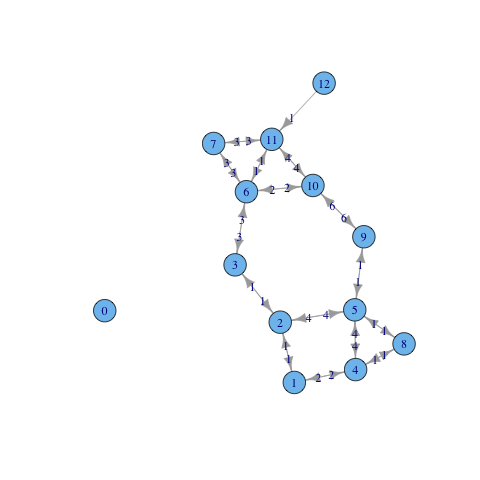
\includegraphics[scale=.5]{test_network.png} 
\caption{Lyhyimmän polun etsimiseen käytetty testiverkko}
\label{testiverkko}
\end{figure}

Täsmällisesti testit toteutettiin seuraaville tapauksille:

\begin{enumerate}
\item Solmun 0 etäisyys kaikista muista solmuista tulee olla ääretön.
\item Kaikkien muiden solmujen etäisyys solmusta 0 tulee olla ääretön.
\item Etäisyys solmusta 12 solmuun 11 tulee olla 1.
\item Etäisyys solmusta 11 solmuun 12 tulee olla ääretön.
\item Lyhyin reitti solmusta 1 solmuun 5 kulkee solmujen 4 ja 8 kautta, ja muodostetun reitin pituus on 4.
\item Lyhyin reitti solmusta 5 solmuun 6 kulkee solmujen 2 ja 3 kautta, ja muodostetun reitin pituus on 8.
\item Lyhyin reitti solmusta 1 solmuun 11 kulkee solmujen 2, 3 ja 6 kautta, ja muodostetun reitin pituus on 6.
\item Lyhyin reitti solmusta 4 solmuun 5 kulkee solmun 8 kautta, ja muodostetun reitin pituus on 2.
\label{network_test}
\end{enumerate}

Testit on toteutettu abstraktille yläluokalle \texttt{ShortestPathGraph}, jolloin samaa testikoodia voidaan käyttää sekä luokille \texttt{AStarPathGraph} sekä \texttt{DikstraPathGraph}. Kun testataan A*-implementaatiota, on syytä asettaa heuristiseksi funktioksi nollafunktio, jolloin algoritmi palautuu Dikstan algoritmiksi -- jolle on taattua löytää lyhyin reitti (katso tarkemmin taulukkko \ref{heuristic_correct}).

\section{Evaluaatio}

Ohjelmaa on järkevää evaluoida kahdesta eri näkökulmasta: ratkaisuiden oikeellisuus sekä suoritusaika. Kuten yllä mainittiin, sekä Dikstran algoritmi että A*-toteutus heuristisella funktiolla $h(v_x,v_g) = 0$ toimivat oikein. Tällöin on mielekästä keskittyä arvioimaan heuristisia funktiota $h'_1( v_x, v_g ) = |\mathcal{G}| - \mathcal{N}( v_x , v_g )$ sekä $ h'_2( v_x, v_g ) = \mathcal{E}_w ( v_x ) \cdot ( |\mathcal{G}| - \mathcal{N}( v_x , v_g ) ) $. Kappaleessa \ref{heuristic_correctness} esitetään yksinkertaisia tuloksia tähän liittyen. Koska kyseessä on tietorakenteiden ja algoritmien harjoitustyö, myös suoritusaika on mielekäs vertailukohta, olen vertaillut Dikstran algoritmia sekä A*-algoritmia kummallakin heuristiikalla luvussa \ref{suoritusaika}.

\begin{table}
\begin{tabular}{l|c|c }
Tapaus & $ |\mathcal{G}| - \mathcal{N}( v_x , v_g )$  & $ \mathcal{E}_w ( v_x ) \cdot ( |\mathcal{G}| - \mathcal{N}( v_x , v_g ) ) $ \\ 
\hline 
1 \& 2 & 0 & 0 \\ 
3 \& 4 & 0 & 0 \\  
5 & 1 & 0 \\
6 & 0 & 0 \\
7 & 0 & 0 \\
8 & 2 & 0 \\
\hline
Väärin & 2 & 0 \\
\hline 
\end{tabular} 
\caption{Heuristiikoiden virheellisyys}
Eri heuristiikoiden virheellisyys, yksikköä. Testit kuvattu sivulla \pageref{network_test}.
\label{heuristic_correct}
\end{table}

\subsection{Heuristiikoiden oikeellisuus}
\label{heuristic_correctness}

Kumpaakin ehdotettua A*-heuristiikkaa testattiin yksinkertaisella testiverkolla (kuva \ref{testiverkko}, kuvaus sivulla \pageref{network_test}). Tämä testaus ei luonnollisestikaan ole kokonaisvaltainen, eikä tuloksen perusteella tulisi päätellä $h'_2$ -heuristiikan olevan parempi kuin $h'_1$. Tämän testaamiseksi olisi välttämätöntä käsitellä laajempia verkkoja ja suorittaa täsmällisempi arvio jokaisesta solmusta jokaiseen solmuun, sekä verrata tuloksia heuristiikoiden kanssa. Testausprosessi voisi siis olla seuraava:

\begin{algorithmic}
\ForAll{$e_1$ in $\mathcal{G}$}
\ForAll{$e_2$ in $\matgcal{G} - e_1$}
\State $correct \gets $ path$_\mathfrak{D}( e_1 , e_2 )$
\State $heuristic_1 \gets $ path$_\mathfrak{A_{H1}}( e_1 , e_2 )$
\State $heuristic_2 \gets $ path$_\mathfrak{A_{H2}}( e_1 , e_2 )$
\EndFor
\EndFor
\end{algorithmic}

Tulos kuitenkin osoittaa heuristisen ratkaisun keskeisen piirteen: vaikka suoritusaikaa pystytään vähentämään, niin ratkaisun tarkkuutta ei tällöin voida taata.

\subsection{Suoritusaika}
\label{suoritusaika}

\bibliographystyle{apalike} 
\bibliography{doc}

\end{document}